\chapter{开放式对比资源接入方法}
本文将数据、模型和对比方法称之为对比资源,这三者的开放性决定了对比结果的准确性、公开性和公平性。其中模型作为对比的对象,是本系统中最重要的要素之一。传统的模型对比方案将模型部署在本地环境运行,针对第\label{sec:scene}节分析的多对比情景需求,会造成难以共享和重现等问题,本章描述的模型服务化封装、部署和发布对此提出了对策;而数据资源作为支撑模型成功运行的必备要素,传统的基于数据拷贝的方式在这种情景下也不能满足要求,因此本章对数据资源的开放式接入也提出了相应的方案;在这两者的基础之上,将统计学对比方法和可视化对比方法也一并接入到框架之下,实现了模型的开放式对比。

\section{开放式碳循环相关数据资源接入方法}
网络空间中的数据按照其组织结构可以分为结构化数据、半结构化数据和非结构化数据,地理模型在运行时强烈依赖于输入数据的结构,所以半结构化和非结构化数据的半结构化描述是数据应用时重要部分。
本节首先从数据格式、尺度、编排三个方面详细地分析了碳循环相关数据资源的特征,对领域通用数据设计了结构化的描述接口,以帮助数据资源介绍、接入、匹配和展示。最后遵循OGC WMS、WFS、WCS标准,使用GeoServer发布碳循环数据服务,实现了空间数据的在线预览和查询检索,对于对比过程中需要进行的数据抽取和重组,设计了数据重构服务以支持他的网络化应用。

\subsection{碳循环相关数据资源结构特征分析}
\subsubsection{数据格式分析}
碳循环相关数据主要有几种格式:NetCDF、CSV、Shapefile和TXT,如表~\ref{tab:data-format-feature}所示,这些数据都是非结构化的。

\begin{table}[H]
    \centering
    \caption{数据格式和特征}
    \label{tab:data-format-feature}
    \begin{threeparttable}
        \begin{tabular}{lll|l}
            \Xhline{1.5pt}
            数据格式 & 数据类型 & 维数 & 数据名称 \\
            \Xhline{1.5pt}
            \multirow{2}{*}{Shapefile} & \multirow{2}{*}{矢量数据} & \multirow{2}{*}{2维} & 网格点 \\
            \cline{4-4}
            & & & 观测站点 \\
            \hline
            \multirow{5}{*}{NetCDF} & \multirow{5}{*}{场数据} & \multirow{5}{*}{n维} & DEM \\
            \cline{4-4}
            & & & MERRA 2 \\
            \cline{4-4}
            & & & Soil \\
            \cline{4-4}
            & & & PFT \\
            \cline{4-4}
            & & & 全球计算结果 \\
            \hline
            \multirow{2}{*}{\makecell{CSV}} & \multirow{2}{*}{二维表} & \multirow{2}{*}{2维} & 网格点输入气象数据 \\
            \cline{4-4}
            & & & 网格点计算结果 \\
            \hline
            \multirow{3}{*}{\makecell{TXT}} & \multirow{3}{*}{文本数据} & \multirow{3}{*}{1维} & CO2浓度 \\
            \cline{4-4}
            & & & PFT \\
            \cline{4-4}
            & & & Biome-BGC的运行配置 \\
            \Xhline{1.5pt}
        \end{tabular}
    \end{threeparttable}
\end{table}

\begin{enumerate}[(1)]
    \item \textbf{NetCDF}
    
    NetCDF(network Common Data Form)网络通用数据格式是由美国大学大气研究协会的Unidata项目科学家针对科学数据的特点开发的,是一种面向数组型并适于网络共享的数据的描述和编码标准,已被作为OGC的一项标准使用。NetCDF数据通常用来表示多维场数据,从数学上来看,它存储的数据就是一个多自变量的单值函数:$f(x,y,z,...)=value$。其中$x,y,z$等在NetCDF中被称为维(Dimension),函数值$value$被称为变量(Variables),维和变量在物理学上的一些性质,被称为属性(Attributes)。当维度只有经纬度时,可以用来表示栅格数据,如本文中的植被功能类型数据、DEM数据、土壤质地数据。维度除了经纬度以外通常还有时间维,如本文中的MERRA 2气象数据和全球范围内的模型计算结果。具体的维度和变量信息如表~\ref{tab:nc-dim-var} % 参考百度百科

    \begin{table}[H]
        \centering
        \caption{NetCDF数据的维度和变量列表}
        \label{tab:nc-dim-var}
        \begin{threeparttable}
            \begin{tabular}{lll}
                \Xhline{1.5pt}
                数据名称 & 维度 & 变量 \\
                \Xhline{1.5pt}
                DEM & 经度、维度 & 高程 \\
                \hline
                MERRA 2 & 经度、维度、时间 & \multicolumn{1}{m{0.4\columnwidth}}{最低温、最高温、平均温、相对湿度、降水、风速、云量} \\
                \hline
                Soil & 经度、维度 & \multicolumn{1}{m{0.4\columnwidth}}{沙粒含量、黏粒含量、粉粒含量} \\
                \hline
                PFT & 经度、维度 & 植被类型编号 \\
                \hline
                全球计算结果 & 经度、维度、时间 & \multicolumn{1}{m{0.4\columnwidth}}{GPP、NPP、NEP、Biomass、ET} \\
                \Xhline{1.5pt}
            \end{tabular}
        \end{threeparttable}
    \end{table}

    \item \textbf{CSV}
    
    CSV(Comma-Separated Values)逗号分隔符文件是以文本形式存储的表型数据。CSV文件由任意数量的记录组成,每行称之为一条记录,每条记录由多个字段组成,字段之间由分隔符分割,通常是逗号或制表符。CSV文件有一系列的规则,比如可以选择性的包含列名,开头不能留空行,每条记录不能跨行等。本文中的CSV文件有网格点气象数据、网格点结果数据和站点观测数据,他们除了具备常规CSV文件的特点以外,还都用一列来表示时间。

    \item \textbf{Shapefile}
    
    Shapefile是ESRI开发的一种矢量空间数据格式,也属于OGC的一项标准。Shapefile文件用点线面描述空间对象的几何信息,用属性表描述对象的属性,另外还包括有数据的空间参考坐标、图形索引等。本文中用到的Shapefile数据是由$0.5^{\circ} \times 0.5^{\circ}$的经纬网划分而来的网格点。

    \item \textbf{TXT}
    
    TXT文件是最常用的文件格式,没有固定的结构。

\end{enumerate}

\subsubsection{数据尺度分析}
尺度是地理学数据的重要特征,指数据集表达的时空范围和精度,不同尺度数据表达的信息密度有很大差异。
\begin{enumerate}[(1)]
    \item \textbf{时间尺度}
    
    主要指数据的时间范围和精度,碳循环的数据和模拟有很强的多样性,精度上可细分为日尺度、月尺度、季节尺度、年尺度、百年尺度等,范围上包括1年、多年甚至几十年。本文的模拟全部在日尺度上进行,模拟时间范围为1982年到2014年,观测数据的时间范围视具体站点而定,一般为1-10年左右。在对比时,由于日尺度的时间序列长度比较大,且数据噪点比较多,因此,也需要对其时间分辨率进行调整,以月尺度、季节尺度和年尺度对其进行平滑,可以提高数据的精度。

    \item \textbf{空间尺度}
    
    主要体现在数据的空间范围和分辨率上。如表~\ref{tab:spatial-multi-resulotion}所示,各种输入数据的分辨率和范围不尽相同,本文统一重采样为$0.5^{\circ} \times 0.5^{\circ}$,并以其划分网格在全球范围内模拟。

    \begin{table}[H]
        \centering
        \caption{碳循环模拟的空间多尺度特征}
        \label{tab:spatial-multi-resulotion}
        \begin{threeparttable}
            \begin{tabular}{lrrrr}
                \Xhline{1.5pt}
                数据名称 & 经度分辨率 & 纬度分辨率 & 北纬边界 & 南纬边界 \\
                \Xhline{1.5pt}
                模拟输入和输出 & $0.5^\circ$ & $0.5^\circ$ & $82.25^\circ$ & $-54.75^\circ$ \\
                MERRA 2 & $0.625^\circ$ & $0.5^\circ$ & $90^\circ$ & $-90^\circ$ \\
                DEM & $0.5^\circ$ & $0.5^\circ$ & $89.75^\circ$ & $-89.75^\circ$ \\
                土壤 & $0.0085^\circ$ & $0.0107^\circ$ & $90^\circ$ & $-90^\circ$ \\
                植被功能类型 & $0.66^\circ$ & $0.5^\circ$ & $90^\circ$ & $-90^\circ$ \\
                MODIS 17 A3 GPP/NPP & $0.0083^\circ$ & $0.0083^\circ$ & $80^\circ$ & $-60^\circ$ \\
                \Xhline{1.5pt}
            \end{tabular}
        \end{threeparttable}
    \end{table}

\end{enumerate}

\subsubsection{数据编排分析}
\label{subsubsec:data-arrange}
由于三个模型对于数据的要求不完全相同,所以合理的数据编排对数据检索、下载、模型运行都是至关重要的。如图~\ref{fig:data-split-map}所示,每套数据集存放在固定的路径下,可由数据库解析到。在运行一个格点时,首先从网格点shapefile的属性表中获取他的编号,再对应到具体的数据集和模型下面,可以获取详细的输入输出文件列表。

\begin{figure}[!htbp]
    \centering
    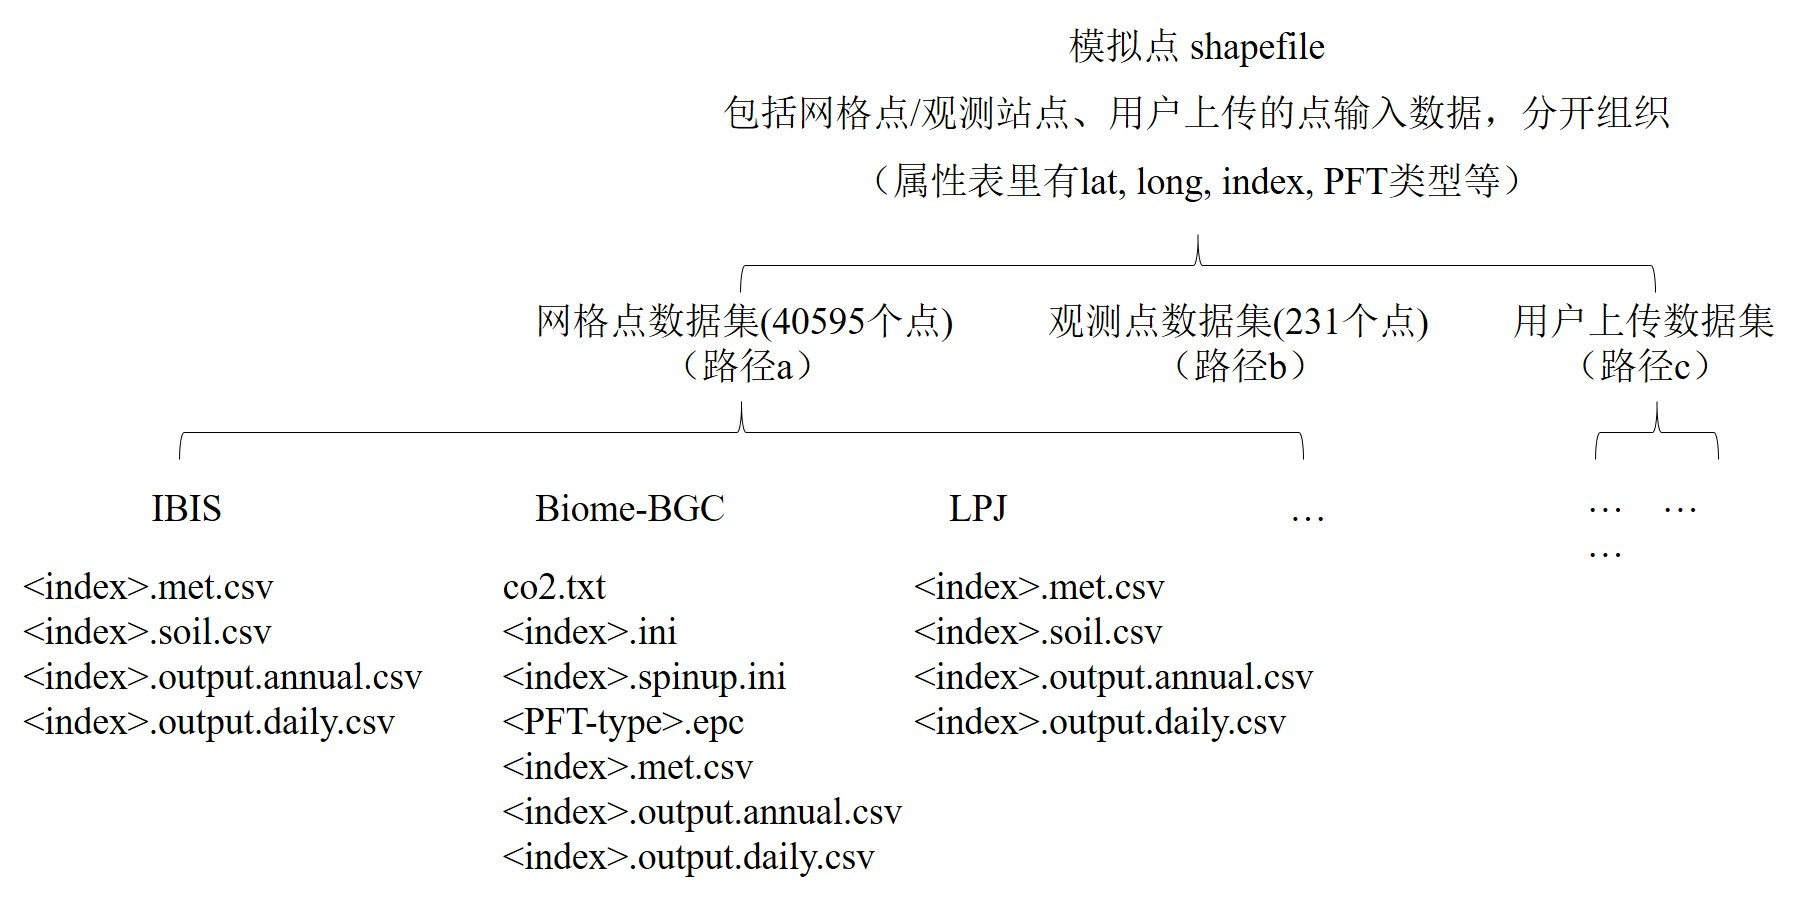
\includegraphics[width=1\textwidth]{data-arrange}
    \caption{陆地生态系统碳循环模型输入数据编排}
    \label{fig:data-arrange}
\end{figure}

\subsection{碳循环相关数据资源描述方法}
\label{sec:data-desc}
元数据是关于数据的数据,它主要描述数据的内容、质量、表示方式、空间参照系、管理方式、数据的所有者、数据的提供方式和数据集的其他特征等。地理信息元数据可以用来管理和维护空间数据,方便查询和检索空问数据,为用户提供数据内容,质量状态和相关特性的数据编目,为地理信息共享提供了基础。对于数据的描述,国内外都有很多对应的研究,OGC采用XML Schema(如GOC Simple Feature规范)来描述GML,来支持WPS的运行~\cite{OGC-WPS}。OpenMI(Open Modelling Interface)设计了一套标准接口用于多模型集成耦合时对数据的定义、描述和传递~\cite{MOORE2005279}。乐松山设计的通用数据表达——交换模型(Universal Data Description eXchange Model,UDX),结合数据映射服务和数据重构服务,面向模型集成应用场景可以对数据结构进行结构化、语义化描述~\cite{乐松山2016面向地理模型共享与集成的数据适配方法研究}。

\begin{figure}[!htbp]
    \centering
    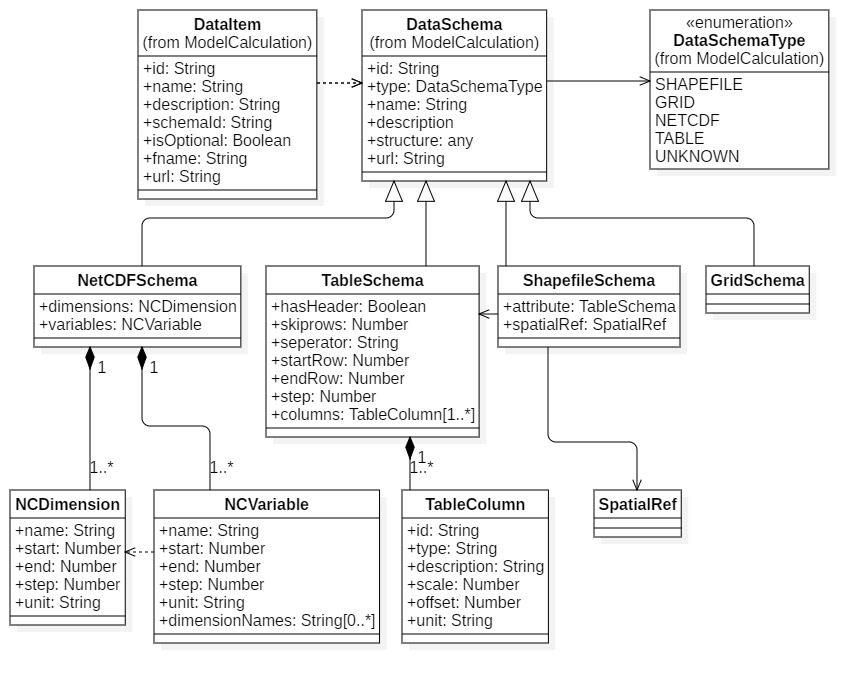
\includegraphics[width=.8\textwidth]{UML-data-description-interface}
    \caption{数据描述接口设计}
    \label{fig:UML-data-description-interface}
\end{figure}

为适应本系统的需求,本文并没有采用这些数据描述标准,而是采用自定义结构进行结构化描述。对于数据的描述分为两部分:领域通用格式数据的描述和自定义结构数据的描述。对于前者,本文设计了如图~\ref{UML-data-description-interface}所示的描述文档,针对每种格式数据各自的特点,以可扩展的形式对其进行描述。对于自定义结构的数据,本文采用示例数据的形式描述。

如图~\ref{fig:data-desc-example},对于Table数据的描述,主要包括解析数据的表头和列信息组成,表头信息包括有无表头、跳过行数、分隔符、起始列号、终止列号、步长信息。列信息包括数据缩放因子、偏移量、描述和单位信息组成。
对于NetCDF数据的描述,包括维度和变量信息。他们都包括名称、缺省值、缩放因子、偏移量等信息。

\begin{figure}[!htbp]
    \centering
    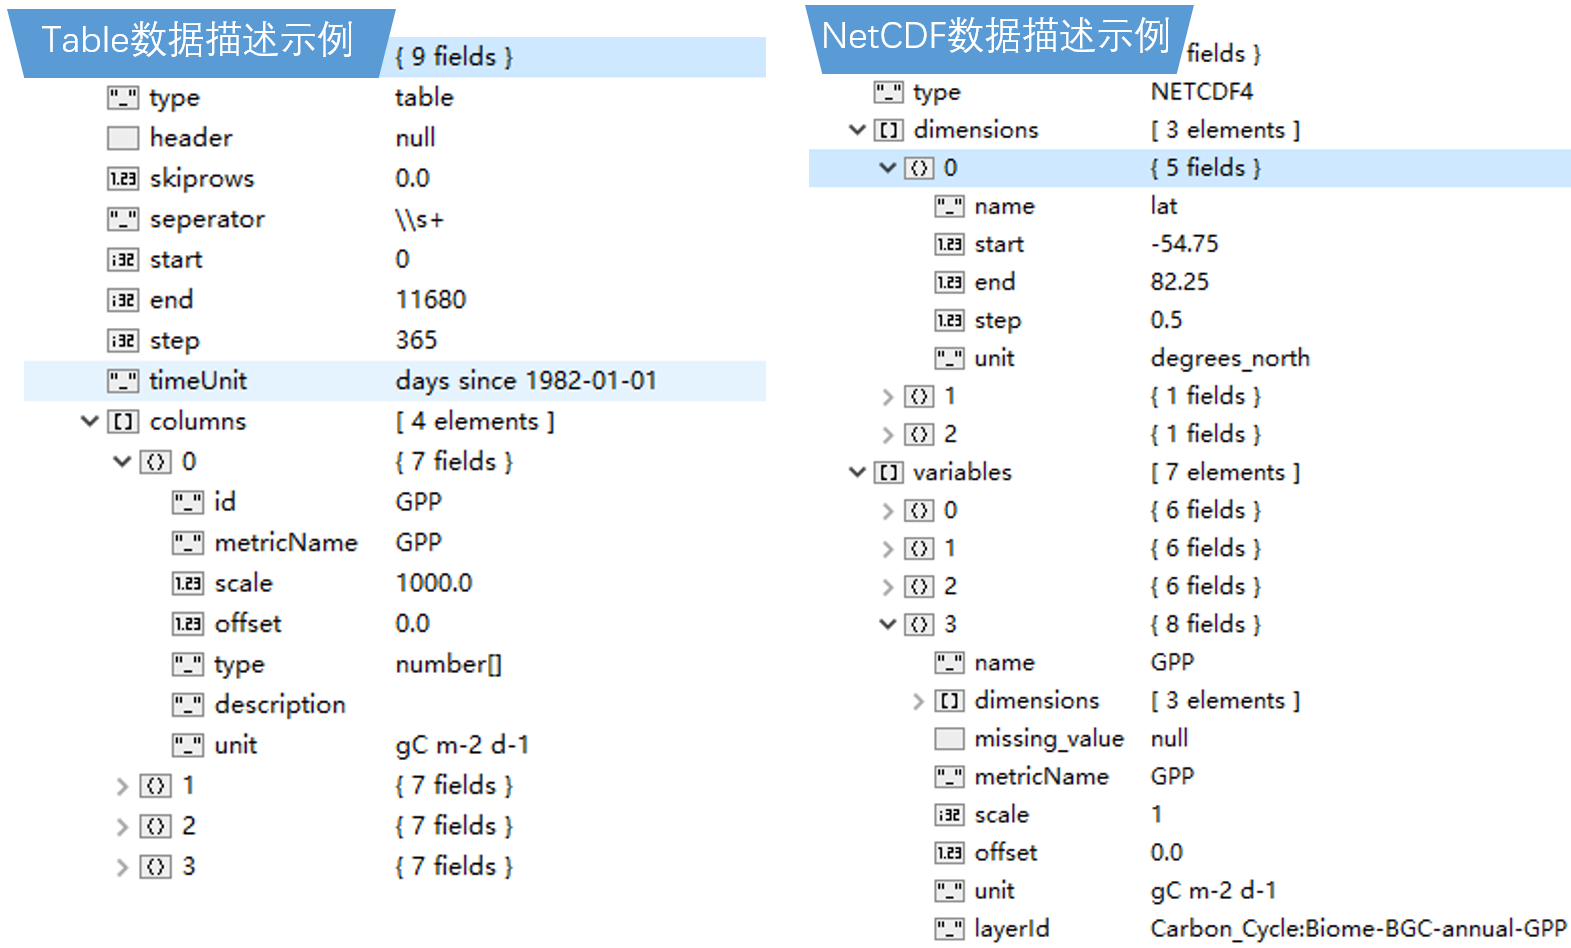
\includegraphics[width=.8\textwidth]{data-desc-example}
    \caption{Table和NetCDF数据描述文档示例}
    \label{fig:data-desc-example}
\end{figure}

\subsection{碳循环相关数据资源的服务化封装}
\subsubsection{WMS、WFS、WCS三种服务的发布}
为实现一套与厂商无关的空间数据互操作规范,开放地理空间信息联盟(OGC)制定了WMS、WFS、WCS服务标准,具体接口如表~\ref{tab:OGC-WMS-WFS-WCS}所示。其中WMS(Web Map Service)利用具有地理空间信息的数据制作地图,在国际规范中,地图是地理数据的可视化表现,WMS返回的地图并非是地图数据,而是地图图像,格式上可以是PNG、GIF、JPEG、SVG等~\cite{OGC-WMS}。WFS(Web Feature Service)通过GML(Geography Markup Language)传递地理空间数据,它支持在基于HTTP协议的分布式计算平台上对地理要素进行增删查改等操作,并在这些操作过程中保证了地理数据变化的一致性~\cite{OGC-WFS}。WCS(Web Coverage Service)在网络上以覆盖(Coverage)的形式共享地理空间数据,能够返回栅格时空范围中任意指定点的值,实现了栅格影像数据集的共享~\cite{OGC-WCS}。
本文将网格点的Shapefile发布为WFS,通过界面上的交互查询到选择的格点要素,解析其属性后可以获取输入数据路径。将全球范围下的计算结果和对比结果NetCDF数据发布为WMS和WCS,可以在线查看和下载。

\begin{table}
    \centering
    \caption{OGC WMS、WFS、WCS接口}
    \label{tab:OGC-WMS-WFS-WCS}
    \begin{threeparttable}
%        \begin{tabular}{ l | l p{0.5\columnwidth}} 
        \begin{tabular}{ l | l l}
            \Xhline{1.5pt}
            类型 & 接口 & 描述 \\
            \Xhline{1.5pt}
            \multirow{3}{*}{WMS} & GetCapabilities & \multicolumn{1}{m{0.6\columnwidth}}{返回服务级元数据,包括对服务信息内容和可接受请求参数的描述} \\
            \cline{2-3}
            & GetMap & 返回一幅地图影像 \\
            \cline{2-3}
            & GetFeatureInfo & 返回地图上要素的空间实体信息 \\
            \hline
            \multirow{5}{*}{WFS} & GetCapabilities & 返回服务级元数据 \\
            \cline{2-3}
            & DescribeFeatureType & 返回表示要素结构的XML文档 \\
            \cline{2-3}
            & GetFeature & 返回GML形式的要素实例 \\
            \cline{2-3}
            & Transaction & 增删查改事务请求 \\
            \cline{2-3}
            & LockFeature & 在事务期间对一个或多个要素实例上锁 \\
            \hline
            \multirow{3}{*}{WCS} & GetCapabilities & 返回描述服务和数据集的XML文档 \\
            \cline{2-3}
            & DescribeCoverage & 返回对覆盖的详细描述 \\
            \cline{2-3}
            & GetCoverage & 使用覆盖格式(图片)返回地理位置的值或属性 \\
            \Xhline{1.5pt}
        \end{tabular}
        \begin{tablenotes}
            \footnotesize
            \item 详细接口参考OGC~\cite{OGC-WMS}~\cite{OGC-WFS}~\cite{OGC-WCS}。
        \end{tablenotes}
    \end{threeparttable}
\end{table}

\subsubsection{数据下载服务}
数据下载服务主要是针对图~\ref{fig:data-arrange}设计的数据编排方式,在数据下载时,对数据路径进行反编码,查询到具体的数据条目,并通过HTTP协议返回给用户。

\subsubsection{数据处理服务}
% schema 匹配
% 数据抽取
% 数据重组
% 单位量纲
如图~\ref{fig:data-process-service}所示,本文用到的数据处理服务有三个:
\begin{enumerate}[(1)]
    \item \textbf{单位量纲转换服务}
    
    IBIS、Biome-BGC、LPJ三个模型的输出项单位不完全相同,比如GPP的单位有$gC \cdot m^2/d$、$kgC \cdot m^2/d$、$kgC \cdot m^2/a$等,单位量纲转换服务以单位量纲资源库为参考,对三个模型输出数据项进行统一单位。

    \item \textbf{数据抽取服务}
    
    模型输出的数据步长是1天,而观测数据的时间范围往往有1-10年,时间序列过长,而且日间隔的数据噪点过多,通过数据抽取服务可以将其抽取为步长为1月的数据。
    
    \item \textbf{数据重组服务}
    
    模型输出数据是网格点的CSV数据,对于全球范围的数据可视化处理起来不够方便,因此使用数据重组服务将全球40595个格点的数据重组到一起,得到一个NetCDF数据。

\end{enumerate}

\begin{figure}[!htbp]
    \centering
    \subcaptionbox{单位量纲转换服务}{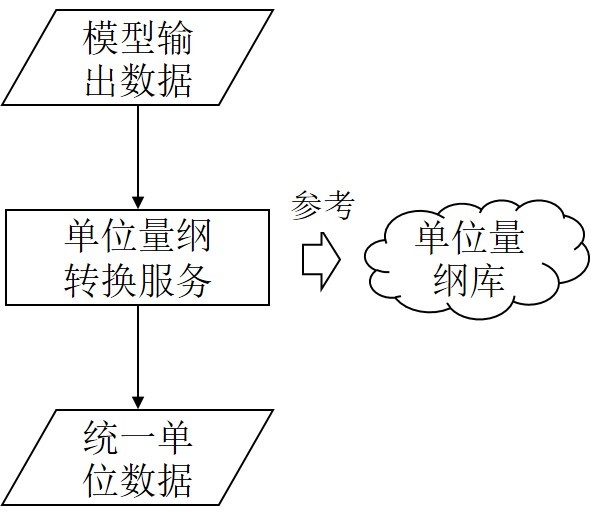
\includegraphics[width=0.4\textwidth]{data-service-1}}
    \hfill
    \subcaptionbox{数据抽取服务}{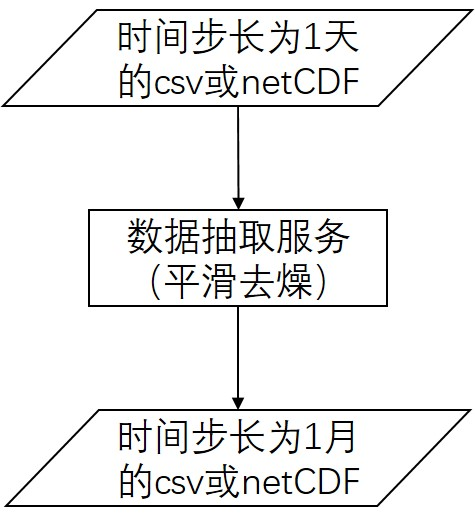
\includegraphics[width=0.25\textwidth]{data-service-2}}
    \hfill
    \subcaptionbox{数据重组服务}{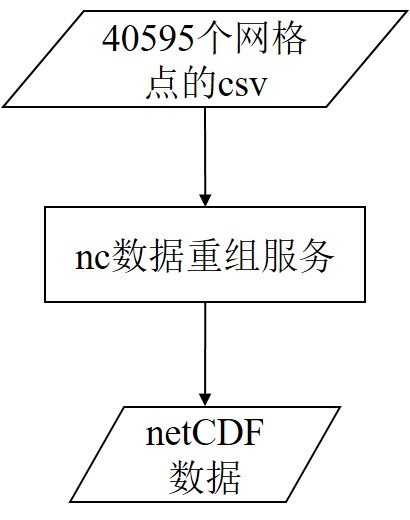
\includegraphics[width=0.25\textwidth]{data-service-3}}
    \caption{数据处理服务}
    \label{fig:data-process-service}
\end{figure}


\section{开放式碳循环模型资源接入方法}
% 从支撑模型运行的角度出发,并结合地理模型对比的需求,梳理了地理模型的运行特征,并以结构化的文档描述模型资源,
% 如图~\ref{ms-join-in}所示,模型资源的接入主要由服务定义、服务封装和服务部署三步组成。

% \begin{figure}[!htbp]
%     \centering
%     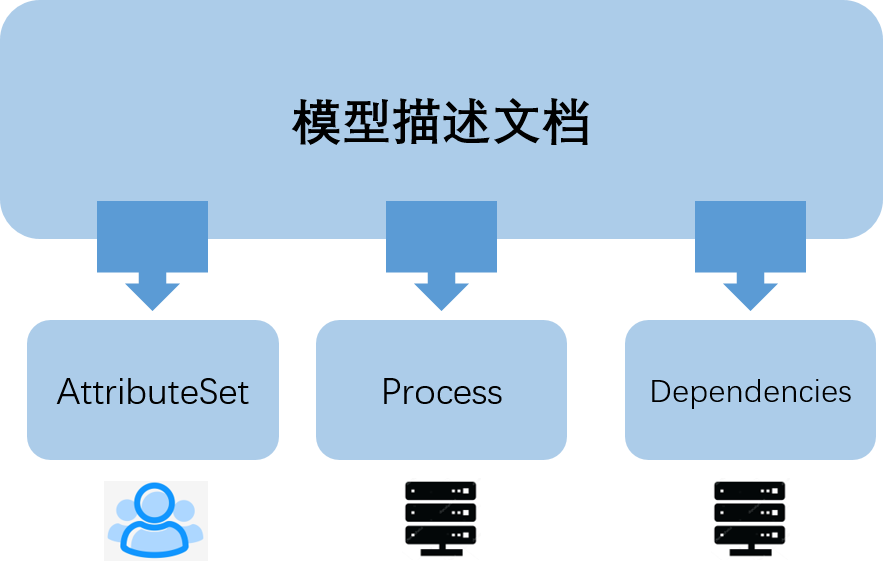
\includegraphics[width=1\textwidth]{mdl}
%     \caption{模型服务的封装、部署和应用}
%     \label{fig:ms-join-in}
% \end{figure}

\subsection{碳循环模型资源特征分析}
% 运行分类:简单型、时间推进型、条件语句型、多子过程的集成
% 运行进度
\begin{enumerate}[(1)]
    \item \textbf{模型参数策略特征}
    
    生态过程模型普遍采用植被功能类型(PFT)作为植被基本处理单元,通常将PFT划分为林地(覆盖热带、温带、寒带,常绿、落叶、针叶和阔叶等)、灌木(常绿和落叶等)、草地($C_3$、$C_4$等)、农田(水稻、玉米、温带谷物、大豆、热带根系作物、太阳花、花生、油菜等)等类型。每种植被功能类型对应有许多植被生理生态参数。

    \item \textbf{模型异构性分析}
    
    地理模型从开发视角上有很多不同的分类体系,如表~\ref{tab:model-language-classify}所示,这些类别中,本文暂不考虑有用户交互的模型。

    \begin{table}
        \centering
        \caption{开发视角上的模型分类}
        \label{tab:model-language-classify}
        \begin{threeparttable}
            \begin{tabular}{l | l l}
                \Xhline{1.5pt}
                分类标准 & 一级分类 & 二级分类 \\
                \Xhline{1.5pt}
                \multirow{8}{*}{语言} & \multirow{5}{*}{编译型} & C \\
                & & C++ \\
                & & C\# \\
                & & Fortran \\
                & & Java \\
                \cline{2-3}
                & \multirow{3}{*}{解释型} & Python\\
                & & MATLAB \\
                & & JavaScript \\
                \hline
                \multirow{3}{*}{平台} & Windows & \\
                & Linux & \\
                & Unit & \\
                \hline
                \multirow{3}{*}{交互} & 无交互 & \\
                & 图形用户界面交互 & \\
                & 控制台用户界面交互 & \\
                \hline
                \multirow{2}{*}{表现形式} & 源代码 & \\
                & 可执行程序 & \\
                \Xhline{1.5pt}
            \end{tabular}
        \end{threeparttable}
    \end{table}

\end{enumerate}


\subsection{碳循环模型资源描述方法}
\label{sec:ms-desc}
模型服务的描述方法是模型服务化的基础。模型服务描述文档应该是面向人的,通过模型服务描述文档提供的信息,模型服务使用者就能够方便地了解和使用模型,并能够理解模型的返回结果;同时模型服务描述文档又是面向机器的,通过模型服务描述文档提供的模型运行输入输出选项,能够判断出模型运行数据的完备性,并在用户发送请求时将模型调用起来。因此,本文将模型服务的描述文档设计为如图~\ref{fig:mdl}。其中AttributeSet表示基本信息描述接口,面向人的理解;Beheavior表示模型的运行行为接口,面向机器理解模型的运行接口;Runtime表示模型的软硬件环境依赖,也是面向机器,表示模型所依赖的软硬件环境信息,从而支持模型能够成功调用起来。
模型服务描述的难点在于对于模型依赖数据的结构的有效表达和对于运行输入输出的合理描述。对于前者,本文采用第~\ref{sec:data-desc}的方法,即采用领域通用标准数据的描述加上示例数据具体展示的形式,对于后者,将在第~\ref{sec:io-interface}节介绍。


模型描述文档由JSON形式表达,与本文选择的具体技术体系有关:一方面它与MongoDB数据库结构同构,可以直接存储于数据库中,有助于增删查改,另一方面它与后台服务器Node.js天生兼容,解析起来方便。

\begin{figure}[!htbp]
    \centering
    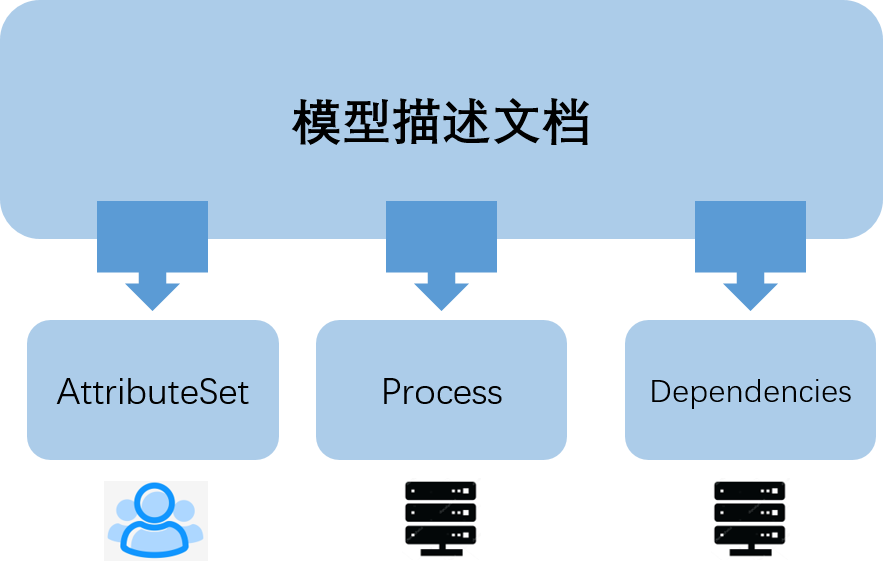
\includegraphics[width=.8\textwidth]{mdl}
    \caption{模型描述文档设计}
    \label{fig:mdl}
\end{figure}

\begin{enumerate}[(1)]
\item \textbf{基本信息描述接口设计}

基本信息的描述如图~\ref{fig:UML-model-description-interface}所示,包括模型名称、作者、关键字、所属分类体系、DOI、wiki和计算节点信息。其中计算节点信息描述了模型服务的IP、端口和路由前缀等信息,从而在模型请求时能够解析出对应的URL。而wiki的设定允许模型服务使用者也能够维护模型服务的介绍,在经过模型服务拥有者的审核后,会补充到模型服务的描述文档中,这样就可以弥补描述接口的不足之处。

\begin{figure}[!htbp]
    \centering
    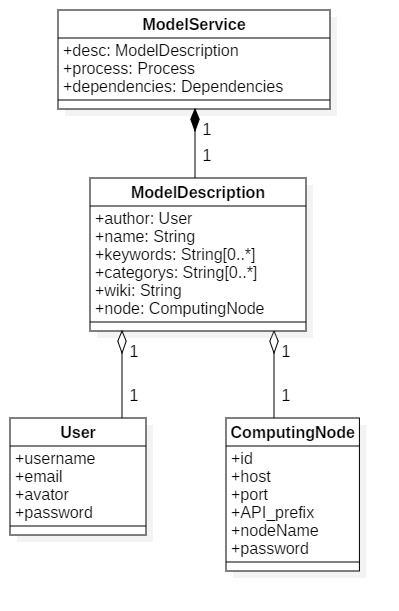
\includegraphics[width=.8\textwidth]{UML-model-description-interface}
    \caption{基本信息描述接口设计}
    \label{fig:UML-model-description-interface}
\end{figure}

\item \textbf{运行信息描述接口设计}
\label{sec:io-interface}
% 存储路径、文件名、类型(编译、解释)、
% 两个粒度:单模型运行和多模型集成

运行信息的描述接口如图~\ref{fig:UML-model-invoke-interface}所示,包括模型的可执行程序文件名、程序类型、解释器类型、输入数据、输出数据和参数以及各种数据的结构化元数据描述。本文将模型从开发语言上分为编译型和解释型两种,对于解释型的语言,需要记录模型的解释器,在运行时通过解释器调用才能运行。通过运行信息的描述,可以在用户调用时执行execute()函数,并返回子进程的pid,在需要时可以通过kill(pid)杀死进程。

\begin{figure}[!htbp]
    \centering
    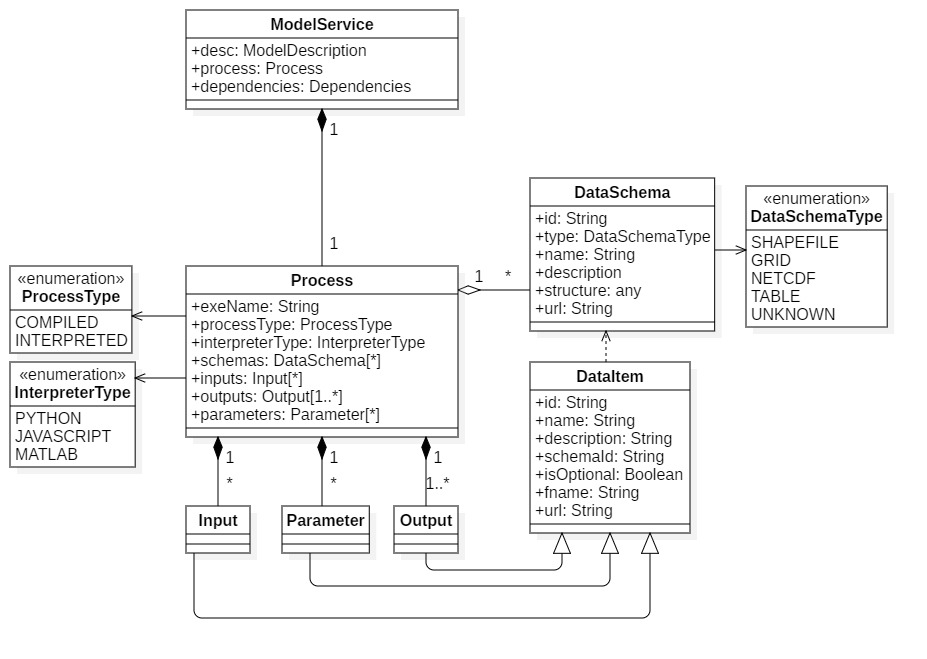
\includegraphics[width=1.1\textwidth]{UML-model-invoke-interface}
    \caption{运行信息描述接口设计}
    \label{fig:UML-model-invoke-interface}
\end{figure}

\item \textbf{部署信息描述接口设计}

部署信息的描述接口如图~\ref{fig:UML-model-deployment-interface}所示,包括模型运行所需的软件和硬件依赖环境。通过与计算节点的软硬件环境数据库相匹配可以得到部署环境是否匹配,当环境相匹配时才能调用成功。

\begin{figure}[!htbp]
    \centering
    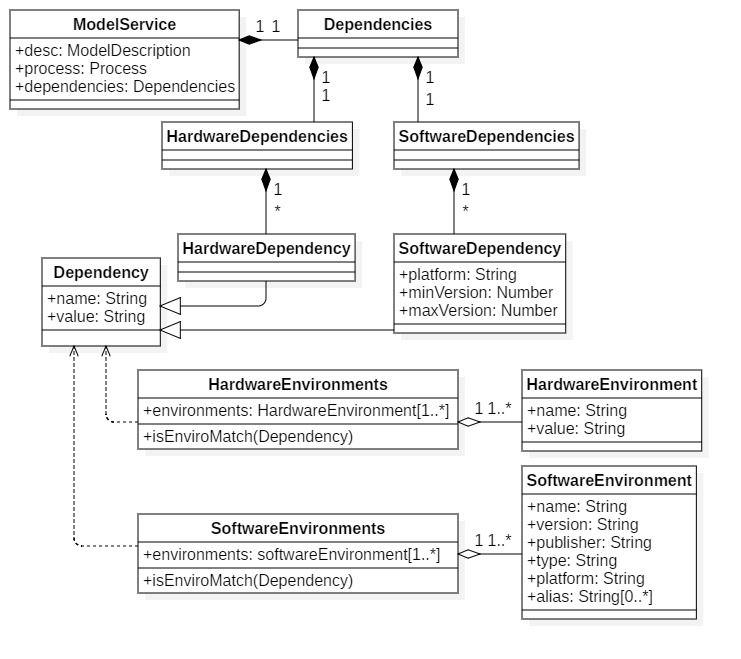
\includegraphics[width=1\textwidth]{UML-model-deployment-interface}
    \caption{部署信息描述接口设计}
    \label{fig:UML-model-deployment-interface}
\end{figure}
\end{enumerate}

\subsection{碳循环模型资源的封装、部署、发布}

\subsubsection{服务封装}
% 接口设计
% 几种方式:模型代理、源码封装
% 对于执行链的封装
在计算机领域,封装是对实体进行包装或组合形成具有稳定接口的新实体的方法和技术。~\cite{胡迪2015地理模型的服务化封装方法研究}通过封装,可以屏蔽原有程序的实现细节,提高模型的可复用性和可维护性,降低用户的使用难度。封装可以体现在程序设计的各个层次上,如函数、类、模块、组件、系统、可执行程序和Web服务这些粒度上都可以进行封装,本文的封装将模型包装成具有标准接口的控制台应用程序。

模型封装最关键的是运行接口的设计,而模型运行接口的设计本质上是设计一个命令行参数解析标准,将输入输出选项映射给程序内存变量,业界有很多成熟的标准,如libc的getopt/getopt\_long接口、google的gflags接口等。本文采用的getopt/getopt\_long接口,它在很多其他语言上都有对应的移植版本,方便对不同语言模型封装的实现。getopt/getopt\_long接口支持单字符选项、多字符选项和可选参数选项,可以方便地生成帮助信息。通过getopt/getopt\_long的标准化,模型的调用命令可表示为“exeName -a -i="filepath1" -p="10" -o="filepath3"”或“exeName -a --inputFile1="filepath2" --parameter1="10" --outputFile1="filepath3"”。其中选项列表来自于运行信息描述文档,以“-”开头表示单字符选项,以“--”开头表示多字符选项,不带等号的如“-a”为参数选项。对于IBIS的封装,标准化后调用方式可表示为“IBIS --meteorology="meteorology\_file\_path" --soil="soil\_file\_path" --output="output\_file\_save\_path"”。对于解释型的语言,需要在命令前面加上解释器,如Biome-BGC模型的调用方式可表示为“node Biome-BGC.js -a --ini="ini\_config\_path" --met="meteorology\_file\_path" --co2="co2\_file\_path" --epc="PFT\_parameters\_file\_path" --output="output\_file\_path"”。

模型封装根据有无源码可以分为源码封装和模型代理封装,如图~\ref{fig:source-encap-proxy-encap}所示,源码封装直接对模型输入输出接口做出修改使其标准化,模型代理封装通过写一个模型代理壳将IO标准化,然后通过子进程启动模型完成封装。按照模型是否包含集成分为简单模型封装和包含集成流程的模型的封装。Biome-BGC模型的执行过程包括spin-up模式和正常模式,整个运行过程中有一个简单的串联集成过程,如图~\ref{fig:ms-encap-with-integration}所示,正常模式的运行依赖于spin-up模式,通过Node.js脚本可以非常方便的串联集成。

\begin{figure}[!htbp]
    \centering
    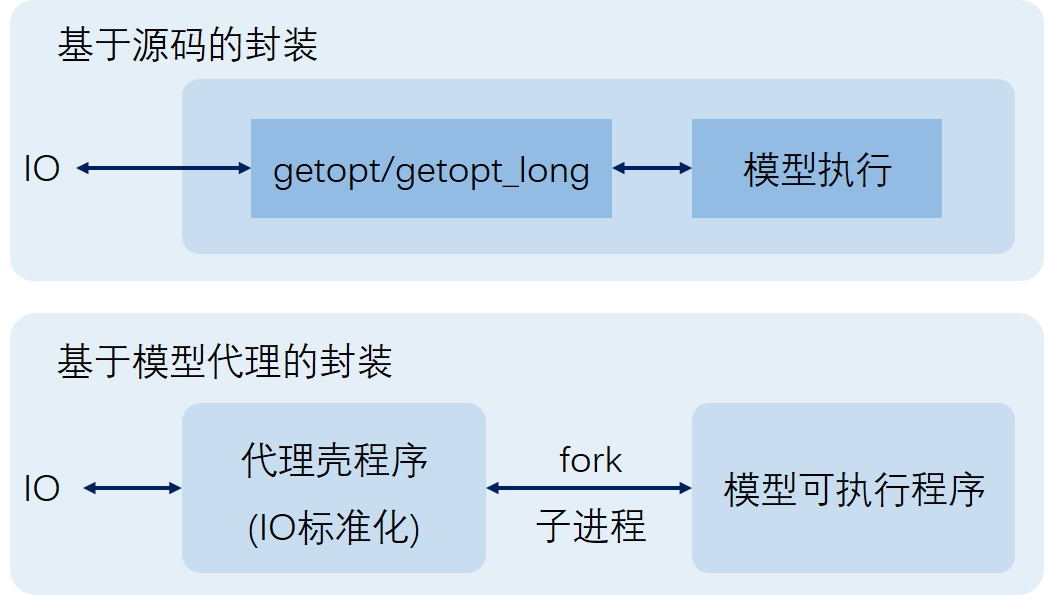
\includegraphics[width=1\textwidth]{source-encap-proxy-encap}
    \caption{源码封装和模型代理封装}
    \label{fig:source-encap-proxy-encap}
\end{figure}

\begin{figure}[!htbp]
    \centering
    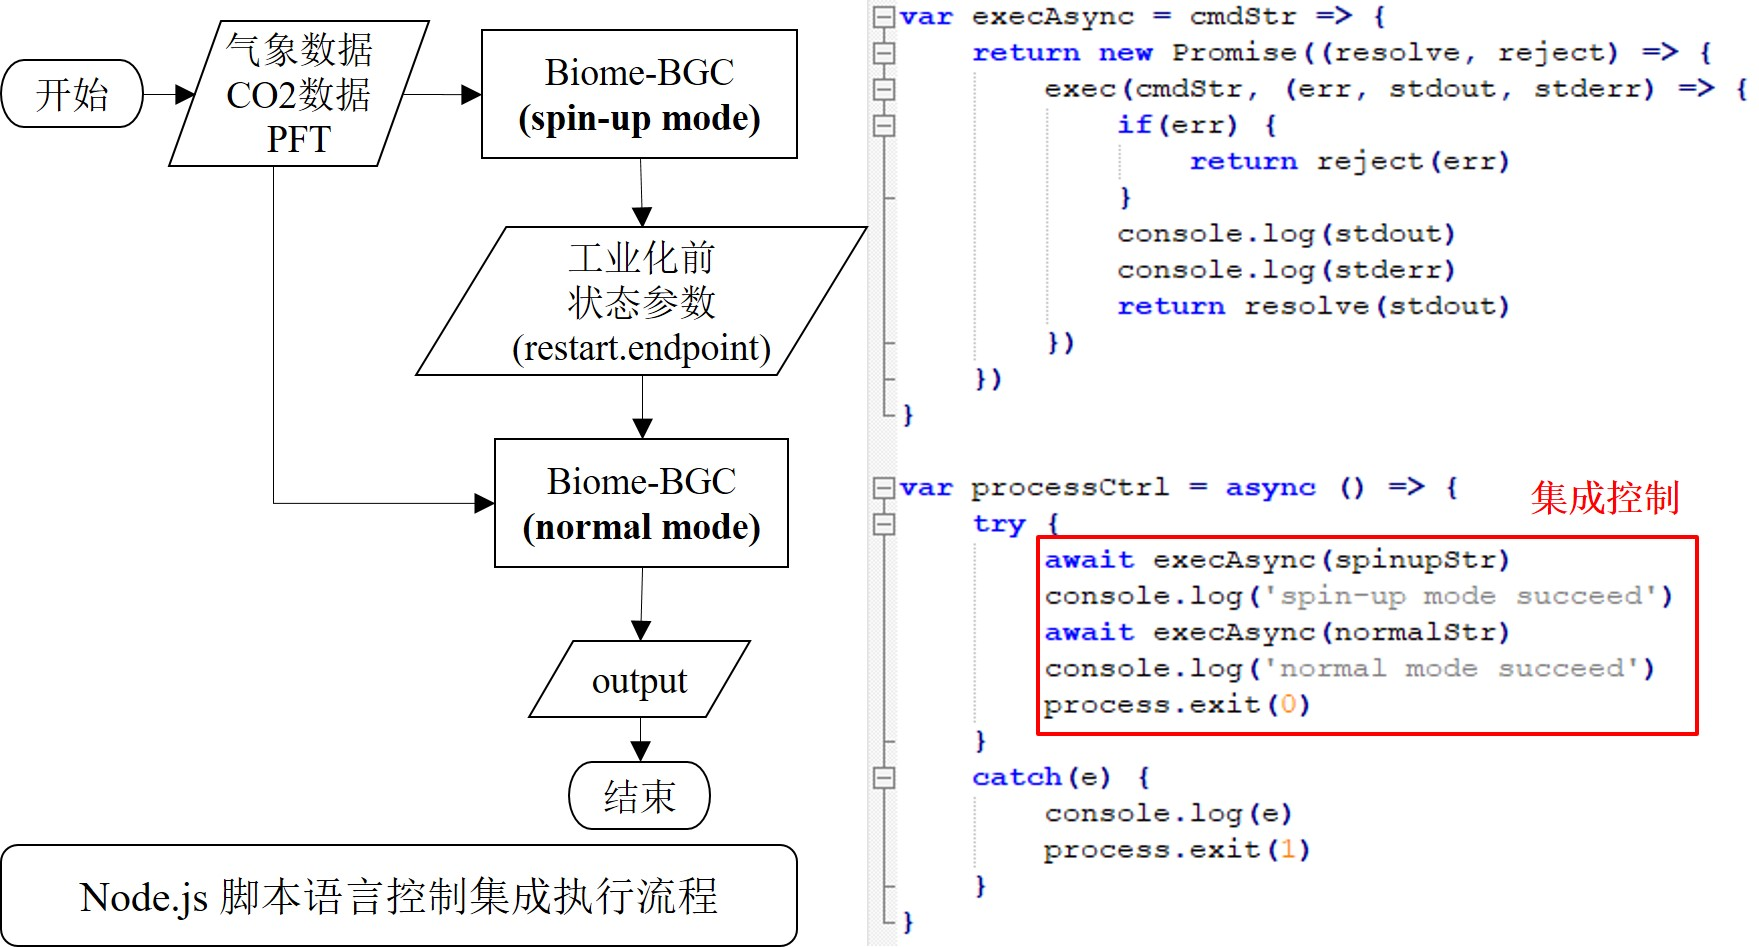
\includegraphics[width=1\textwidth]{ms-encap-with-integration}
    \caption{模型的串联集成封装,以Biome-BGC为例}
    \label{fig:ms-encap-with-integration}
\end{figure}

\subsubsection{服务部署和发布}
% 数据库录入条目、服务部署
% 运行环境
服务部署和发布是将封装好的模型程序迁移到目标计算节点上的过程,主要包括模型服务描述文档数据库条目的录入和模型运行软硬件环境的匹配。对于模型服务描述文档,本文将数据库设计与第\ref{sec:ms-desc}节的描述接口同构,可以直接录入。对于软件环境。。。。对于硬件环境,本文所用的三个模型对硬件要求都不高,可以直接部署在普通PC机上。

\section{开放式碳循环模型对比方法}

\subsection{碳循环模型对比方法}
\subsubsection{统计学对比方法}
\begin{align}
    &SD = \sqrt{\frac{\sum\nolimits_{i=1}^{N}\left(x_i-\bar{x}\right)^2}{N}}
    \label{eq:SD} \\
    &MSE = \frac{\sum\nolimits_{i=1}^{N}\left(y_i-Y_i\right)^2}{N}
    \label{eq:MSE} \\
    % &MSE_S = \frac{}{N}
    % \label{eq:MSE-S} \\
    % &MSE_U = \frac{}{N}
    % \label{eq:MSE-U} \\
    &RMSE = \sqrt{MSE} = \sqrt{\frac{\sum\nolimits_{i=1}^{N}\left(y_i-Y_i\right)^2}{N}}
    \label{eq:RMSE}  \\
    % &RMSE_r = \sqrt{\frac{\sum\nolimits_{_i=1}^{N}\left[\left(y_i-Y_i\right)/\bar{y}\right]^2}{N}} \times 100\%
    % \label{eq:RMSE-R} \\
    % &R^2 = 1 - \frac{\sum\nolimits_{i=1}^{N}\left(y_i-Y_i\right)^2}{}
    % \label{eq:R^2}
    &NSE = 1 - \frac{\sum\nolimits_{i=1}^{N}\left(y_i-Y_i\right)^2}{\sum\nolimits_{i=1}^{N}\left(Y_i - \bar{Y}\right)^2} 
    \label{eq:NSE}
\end{align}
本文主要用以下几个统计变量评价IBIS、Biome-BGC、LPJ三个模型在网格点的模拟准确度:
\begin{enumerate}[(1)]
\item \textbf{标准差(Standard Deviation,记为$SD$)}

标准差又称均方差,用来表示一组数据的离散程度,如公式~\ref{eq:SD}所示。

\item \textbf{均方根误差(Root Mean Square Error,记为$RMSE$)}

均方根误差又称标准误差,表示有限观测数据中,观测值与真值的偏差。本文使用均方根误差表示网格点模拟值与观测值的偏差,从而反映模型的模拟能力。均方根误差可表示为公式~\ref{eq:RMSE},其中$RMSE$表示均方根误差,$MSE$表示均方误差,$y_i(i=1,2,...,N)$为模拟数据,$Y_i$为观测数据。

\item \textbf{效率系数(Nash-Sutcliffe coefficient,记为$NSE$)}

效率系数用来评价模型模拟的好坏~\cite{gordon2003climate},如公式~\ref{eq:NSE}所示,$NSE$等于1减去均方误差与观测值变异的比值。$NSE$值的范围从负无穷大到1,越接近1表示模型效果越好。如果模拟值的均方误差与观测值的方差相同,则$NSE$等于0;如果模拟值的均方误差大于观测值的方差,则$NSE$小于0;如果模拟值的均方误差小于观测值的方差并趋近于后者,则$NSE$趋近于1,表示模型具有很好的模拟能力。

\item \textbf{超级集合}

超级集合由Krishnamuti~\cite{krishnamurti1999improved}等提出,通过多元线性回归分析对每个观测站点的数据进行分析,各模型的权重系数,如公式~\ref{eq:SE}所示:

\begin{align}
    &F_t = \bar{O} + \sum\nolimits_{i=1}^{N}a_i\left(F_{i,t}-\bar{F_t}\right)
    \label{eq:SE}
\end{align}

式中,$F_t$是超级集合合成后的预测值;$\bar{O}$是训练期的平均观测值;$F_{i,t}$是第$i$个模型的预测值;$\bar{F_t}$是第$i$个模式在训练期的平均预测值;$n$是参加建立超级集合的模型数量;$t$是时间;$a_i$是回归系数,代表各个模型的权重。在建立超级集合时,将数据分成训练集和验证集,通过训练集获取式中的各个参数,通过验证集验证超级集合的模拟水平。本文中参与建立超级集合的模型有MODIS MOD17 A3、IBIS、Biome-BGC、LPJ,观测值数据是FLUXNET La Thuile,具体对比结果在第。。。节介绍。

\end{enumerate}

\subsubsection{可视化对比方法}
\begin{figure}[!htbp]
    \centering
    \subcaptionbox{泰勒图\label{fig:example-taylor}}{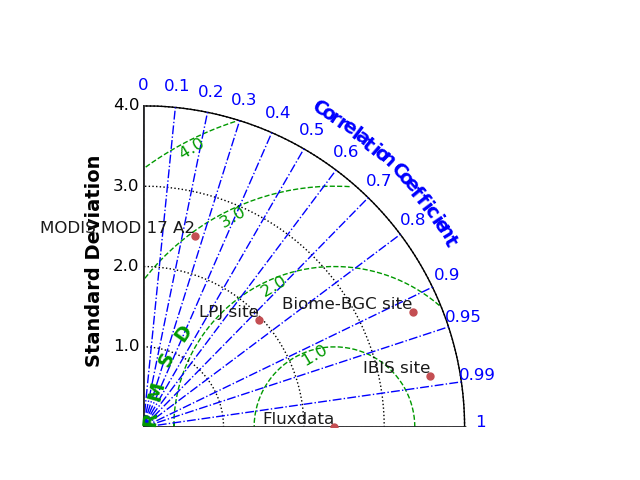
\includegraphics[width=0.47\textwidth]{example-taylor}}
    \hfill
    \subcaptionbox{时间序列折线图\label{fig:example-timeseries-diagram}}{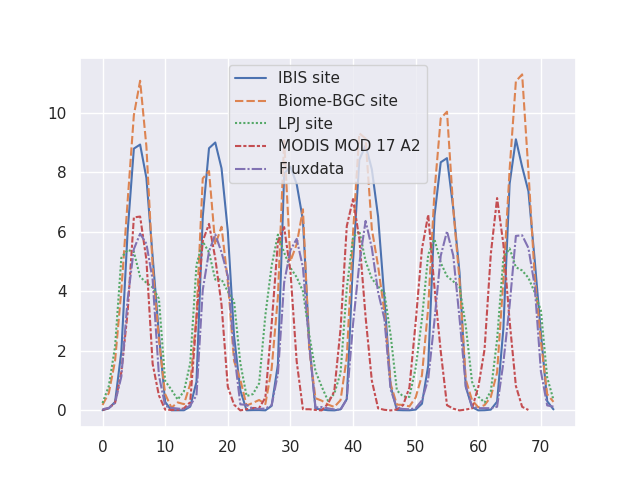
\includegraphics[width=0.47\textwidth]{example-timeseries-diagram}} \\
    \subcaptionbox{热力图\label{fig:example-heatmap}}{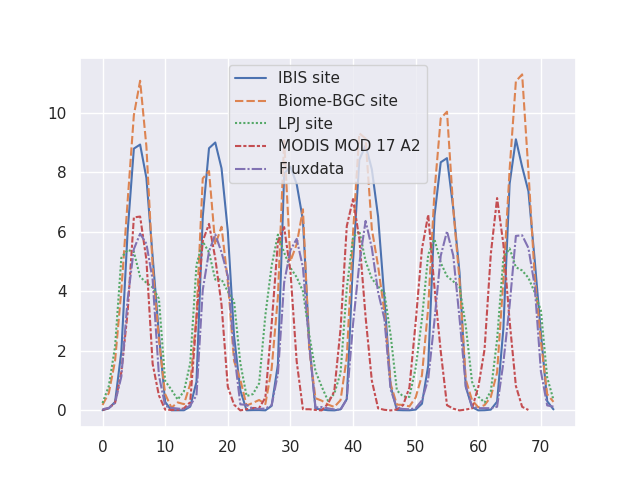
\includegraphics[width=0.47\textwidth]{example-timeseries-diagram}} \\
    \subcaptionbox{等值线图\label{fig:example-contour}}{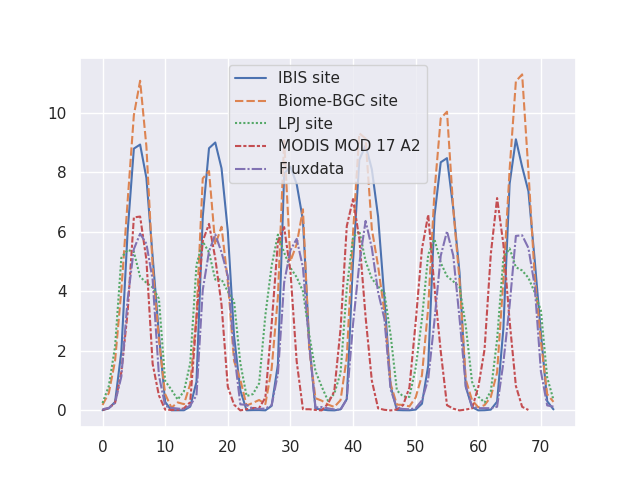
\includegraphics[width=0.47\textwidth]{example-timeseries-diagram}}
    \hfill
    \subcaptionbox{偏差等值线图\label{fig:example-bias-contour}}{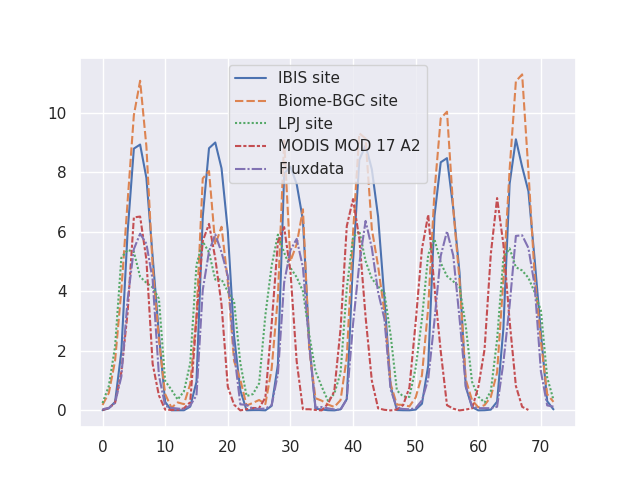
\includegraphics[width=0.47\textwidth]{example-timeseries-diagram}}
    \caption{可视化对比图表}
    \label{fig:ms-server-microservice}
\end{figure}
\begin{enumerate}[(1)]
\item \textbf{泰勒图}
% 全部时间范围,每年的序列

泰勒图常用于评价模型的精度,如图~\ref{fig:example-taylor}所示,泰勒图中的散点表示模型,辐射线表示相关系数,横轴线表示标准差,虚线表示均方根误差~\cite{taylor2001summarizing},泰勒图能够在二维平面上同时呈现三个指标,在IPCC、CMIP5、CMIP6中被广泛应用于多模型模拟能力评估对比。

\item \textbf{时间序列折线图}

如图~\ref{fig:example-timeseries-diagram}所示,时间序列折线图反映的是模拟指标的年度变化趋势,并能够对比模拟值与观测值的趋势差异。

\item \textbf{热力图}
% 按PFT分类

如图~\ref{fig:example-heatmap}所示,横轴是观测站点,纵轴是模型,横着看能直观地发现同一个模型在不同站点的模拟能力差异,纵着看能直观地发现不同模型对同一个站点的模拟能力差异。

\item \textbf{等值线图和偏差等值线图}

如图~\ref{fig:example-contour}和~\ref{fig:example-bias-contour}分别是等值线图和偏差等值线图,等值线图可以直观地表现GPP的空间分布格局,偏差等值线图则表示的是模型误差的空间分布。

\end{enumerate}

\subsection{开放式碳循环模型对比方法接入方法}


\section{本章小结}
本章针对数据、模型和对比方法这三种对比资源在框架下的开放式服务化接入进行了详细的阐述。对于数据资源,从数据格式、尺度、编排三个角度分析了其特征,通过本文设计的结构化描述接口来描述NetCDF、Shapefile和CSV数据,实现了OGC WMS、WFS、WCS、数据下载服务、数据处理服务的发布,为模型成功运行和结果对比提供了基础;对于模型资源,分析了其异构性特征,设计了面向人和机器理解的模型描述接口,并通过运行接口的设计实现了模型服务的封装、部署和发布;对于对比方法,首先详细介绍了本文用到的统计学对比方法和可视化对比方法,在采用模型封装接口将对比方法也封装为开放式服务资源。